\chapter{Equa\cao\ da onda el\'astica}

\section{Teoria Elastodin\^amica}

\subsection{Introdu\cao}

Sob uma carga externa, um corpo pode ser transladado,
rotacionado ou deformado. Na sequ\^encia, estudamos
o efeito chamado de ``deforma\cao''.

A deforma\cao\ de um material \'e um processo no qual
dist\^ancias entre pontos individuais do material s\ao\
alteradas. Em um material real\ih stico, a aplica\cao\
de uma for\ca\ em um lugar particular causa deforma\coes,
primeiro nas proximidades deste lugar e sucessivamente em
partes mais distantes. Este processo \'e chamado de
``propaga\cao\ de onda''.

A propaga\cao\ de onda deve superar a resit\^encia do
material causada pela consist\^encia e a resist\^encia
causada pela in\'ercia. Se a consist\^encia \'e tal que o
material \'e n\ao\ deform\'avel (r\ih gido), o efeito da
aplica\cao\ de for\cas\ externas em um ponto do corpo
poderia ser sentido imediatamente em cada ponto do
material, i.e., o corpo seria movido. Se o material \'e
deform\'avel, ent\ao\ todas as part\ih culas do material
seriam excitadas simultaneamente. N\'os consideramos aqui
um material real\ih stico que \'e deform\'avel e que,
depois de removida a carga, retorna para um estado, que
\'e o mesmo ou similar ao estado antes do carregamento.
Neste \'ultimo caso n\'os falamos sobre materiais
``imperfeitamente el\'asticos'', e no caso anterior sobre
materias ``perfeitamente el\'asticos'', no qual
concentramos nossos estudos.

Uma propaga\cao\ de onda \'e conectada por transmiss\ao\
de energia. A energia \'e transportada de uma part\ih cula
do material para outra, e este transporte n\ao\ \'e pelo
fluxo das part\ih culas. As part\ih culas do material
oscilam ao redor de suas posi\coes\ m\'edias.

Na mec\^anica cl\'assica, o movimento de onda \'e assumido
como uma pequena perturba\cao\ do estado inicial do material,
chamado de ``estado natural''. No estado natural n\ao\ h\'a
tens\oes\ e deforma\coes, ent\ao\ consideramos o estado
natural como sendo o estado de equil\ih brio est\'atico em que a
deforma\cao\ n\ao\ muda com o tempo.

Estudamos aqui como a deforma\cao\ altera rela\coes\ entre
duas part\ih culas pr\'oximas. Esta mudan\ca\
\'e descrita pelo ``tensor de deforma\cao''. Antes
introduzimos o {\it vetor deslocamento}, descrevendo um
deslocamento de uma part\ih cula simples sob uma
deforma\cao. Consideramos para ambos o sistema de
coordenadas cartesianas $x_1$, $x_2$, $x_3$ com origem no ponto 0.

\subsection{Vetor posi\c{c}\~ao}
Seja $P = (x_1,x_2,x_3)$ um vetor que indique a posi\c{c}\~ao de uma part\'icula
no corpo sem deforma\c{c}\~ao e $P'=(x_1',x_2',x_3')$ a posi\c{c}\~ao da
part\'icula no corpo ap\'os a deforma\c{c}\~ao, que estava originalmente em $P$. Perceba que $P$
descreve de maneira \'unica a posi\c{c}\~ao das part\'iculas, e o vetor
\begin{equation}
  P' = P'(P,t)\, ,
\end{equation}
ou
\begin{equation}
  P_i' = x_i'(x_k,t) \quad k=1,2,3 \label{eq:lagrangeana}
\end{equation}
representa a posi\c{c}\~ao das part\'iculas $P$ ap\'os a deforma\c{c}\~ao. 
Esta maneira de descrever o movimento
\'e denominada de descri\c{c}\~ao Lagrangeana ou descri\c{c}\~ao material do
movimento. $P'$ descreve o movimento da perspectiva da part\'icula $P$.
Tomando $t = 0 \equiv t_0$ como o tempo de refer\^encia inicial, temos
que
\begin{equation}
  P'(P,t_0) \equiv P \, .
\end{equation}
Enquanto $P'(P,t)$ \'e a posi\c{c}\~ao atual da part\'icula que estava em $P$ no tempo
$t=0$.

Podemos, tamb\'em, descrever $P$ em fun\c{c}\~ao de $P'$, como
\begin{equation}
  P_i = x_i(x_k',t) \quad k=1,2,3\, . \label{eq:euleriana}
\end{equation}
Essa descri\c{c}\~ao \'e denominada descri\c{c}\~ao Euleriana, ou
descri\c{c}\~ao espacial. Nesta forma, estamos interessados na part\'icula que
ocupa um dado ponto $x_ i'$ no espa\c{c}o no tempo $t$.

\subsubsection{Considera\c{c}\~oes adicionais}
Utilizando a descri\c{c}\~ao euleriana e seja $f'(x_i',t)$ uma fun\c{c}\~ao que
descreve o valor de uma propriedade do meio (e.g., press\~ao, temperatura,
velocidade) em um dado ponto $x_i'$ no tempo $t$. Ao variarmos $t$,
diferentes part\'iculas (identificadas por diferentes valores de $x_i$) ocupam o
mesmo ponto espacial $x_i'$. Vamos nos concentrar em uma \'unica part\'icula
$x_i$. Usando a equa\c{c}\~ao \ref{eq:lagrangeana}, temos
\begin{equation}
  f(x_i,t) = f'(x_k'(x_i,t),t)\, ,
\end{equation}
ou
\begin{equation}
  f(P,t) = f'(P'(P,t),t)\, ,
\end{equation}
onde $f$ e $f'$ n\~ao precisam necessariamente ter a mesma forma funcional. Note
que mantendo $x_i$ fixo e variando $t$, $f'$ \'e uma fun\c{c}\~ao que descreve
o valor da propriedade percebida pela part\'icula que estava inicialmente em $x_i$
e se movimentou no meio.

\subsection{Vetor deslocamento}

Utilizamos a descri\c{c}\~ao Lagrangeana do 
vetor deslocamento $u_i(x_k,t)$ e consideramos uma part\ih cula que, no estado
inicial, est\'a situada no ponto $P=(x_1,x_2,x_3)$. Ap\'os a deforma\cao\
do material, no tempo $t$, esta part\ih cula se encontra
no ponto $P'=(x_1',x_2',x_3')$ (ver figura \ref{fig:vetor-deslocamento}).
A mudan\c{c}a do ponto $P$
para $P'$ \'e especificada pelo ``vetor deslocamento''
%$u_i(x_k,t)$ 
\begin{equation}
u_i(x_k , t)=x'_{i} - x_i ,
\end{equation}
tal que
\begin{eqnarray}
x_i' = x_i + u_i(x_k,t) = x_i + u_i(P,t) \; .
\label{eq:pos-deformacao}
\end{eqnarray}

\begin{figure}[!tb]
\centering
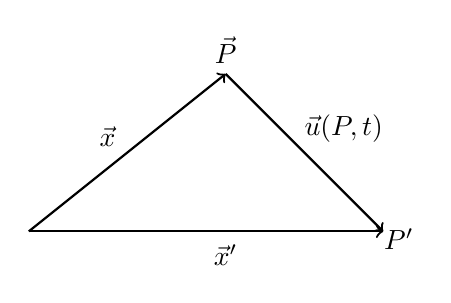
\begin{tikzpicture}
\draw[thick,->] (0,0) -- (4.5,0);% node[anchor=north west] {$P'$};
\draw[thick,->] (0,0) -- (2.5,2);% node[anchor=north west] {$P$};
\draw[thick,->] (2.5,2) -- (4.5,0);% node[above] {$\vec{u}(P,t)$};
\node      (a)         at (1,1.2) {$\vec{x}$};
\node      (b)         at (2.5,-0.3) {$\vec{x}'$};
\node      (c)         at (4.7,-0.1) {$P'$};
\node      (d)         at (2.5,2.3) {$\vec{P}$};
\node      (e)         at (4,1.3) {$\vec{u}(P,t)$};
\end{tikzpicture}
\caption{Representa\c{c}\~ao do vetor deslocamento $\vec{u}(P,t)$.}
\label{fig:vetor-deslocamento}
\end{figure}

Na descri\cao\ Lagrangeana, a velocidade de movimento de
uma part\ih cula \'e dada pela derivada material do vetor posi\cao\ da part\'icula,
ou seja, pela varia\c{c}\~ao temporal do vetor posi\c{c}\~ao da
part\'icula $\bigl(x_i'(x_k,t)\bigr)$, i.e.,
\begin{equation}
  v_i=\left. \frac{Dx_i'}{Dt}\right|_{P fixo} =\left. \frac{\partial x_i'}{\partial t}\right|_{P fixo} \, .
\end{equation}
Assim, calculando a derivada material de $x_i'$, i.e., da equa\cao\ \ref{eq:pos-deformacao}
(visto que $P$ independe do tempo, teremos $\frac{\partial x_i}{\partial t}=0$),
\begin{align}
  \left(\frac{D}{Dt}\right)\,x'_i &= u_i(x_k,t) + x_i \, , \\
  v_i &= \frac{\partial u_i(x_k,t)}{\partial t}\, , \\
  v_i(x_k,t) &= \dot{u}_i(x_k,t) = \frac{\partial u_i(x_k,t)}
{\partial t} \; ,
\end{align}
onde o operador $\frac{D}{Dt}$ indica a derivada material, ou seja, a
varia\c{c}\~ao temporal ``percebida" \hspace{1pt} pela part\'icula.

Similarmente, para a acelera\cao\ da part\ih cula chegamos em
\begin{eqnarray}
a_i(x_k,t) = \ddot{u}_i(x_k,t) = \frac{\partial^2 u_i(x_k,t)}
{\partial t^2} \; .
\end{eqnarray}

A quantidade $v_i(x_k,t)$ \'e conhecida como ``velocidade
da part\ih cula'' e $a_i(x_k,t)$ como a ``acelera\cao\ da
part\ih cula''.

Escolhemos a descri\c{c}\~ao Lagrangeana para simplificar as contas.
para descrevermos a velocidade da part\'icula na perspectiva Euleriana,
escrevemos primeiro o vetor deslocamento, como
\begin{equation}
   u_i(x_k,t)=u_i(x_l'(x_k,t),t) \, .
\end{equation}
Desenvolvendo de maneira similar, temos
\begin{align}
  x_i'&=u_i(x_l'(x_k,t),t) +  x_i \, , \\
  v_i &= \frac{\partial u_i}{\partial x_l'}\frac{\partial x_l'}{\partial t}
  +\frac{\partial u_i}{\partial t} = \frac{\partial u_i}{\partial t} +
  (\vec{v}\cdot\nabla)u_i \, .
\end{align}

\subsection{Tensor de deforma\cao}

Em adi\cao\ ao ponto $P$, n\'os consideramos agora um ponto
$Q=(x_1+dx_1,x_2+dx_2,x_3+dx_3)$ situado nas proximidades do
ponto $P=(x_1,x_2,x_3)$, estando o material ainda n\ao\ deformado. O
ponto $P$ ser\'a movido para o ponto $P'=(x_1',x_2',x_3')$ e o ponto
$Q$ ser\'a movido durante a deforma\cao\ para o ponto
$Q'=(x_1'+dx_1',x_2'+dx_2',x_3'+dx_3')$ (ver figura \ref{fig:tensor-deformacao}). O vetor
deslocamento de $Q$ para $Q'$, $u_i(Q)$, pode ser expresso em termos do
vetor deslocamento $u_i(P)$. Segue, por aproxima\cao\ de Taylor de
primeira ordem, em torno de $x_k$ (uma vez que $dx_i$ \'e supostamente infinitesimalmente
pequeno), que
\begin{eqnarray} \label{vdq}
u_i(Q) = u_i(x_k+dx_k) \approx u_i(x_k) +
\frac{\partial u_i(x_k)}
{\partial x_j} (x_k + dx_j - x_k) \nonumber \\
 = u_i(x_k) +\frac{\partial u_i(x_k)}
{\partial x_j} dx_j = u_i(P) + \frac{\partial u_i(P)}
{\partial x_j} dx_j \; ,
\end{eqnarray}
para todos os pontos $Q$ na vizinhan\ca\ de $P$.


Agora investigamos a mudan\ca\ da dist\^ancia entre os pontos
$P$ e $Q$ devido a deforma\cao. Para isso fazemos a
compara\cao\ do quadrado das dist\^ancias $\overline{PQ}$
e $\overline{P'Q'}$.
Para $\overline{PQ}^2$, n\'os temos
\begin{eqnarray}
\overline{PQ}^2 = dx_i \; dx_i \; .
\end{eqnarray}
Para determinarmos $dx_i'$, observamos (de acordo com a figura \ref{fig:tensor-deformacao}) que
\begin{eqnarray}
dx_i' = dx_i + u_i(Q) - u_i(P) \approx dx_i +
\frac{\partial u_i(P)}{\partial x_j} dx_j \; .
\label{dxidxi}
\end{eqnarray}
expandindo $u_i(Q)$ e usando uma aproxima\c{c}\~ao linear temos
\begin{equation}
  dx_i' \approx dx_i + \frac{\partial u_i(P)}{\partial dx_j}dx_j \, .
\end{equation}


Logo, para $\overline{P'Q'}^2$, temos
\begin{eqnarray}
\overline{P'Q'}^2 = dx_i' \; dx_i' &\approx& \left(dx_i +
\frac{\partial u_i}{\partial x_j} dx_j\right) \left(dx_i +
\frac{\partial u_i}{\partial x_k} dx_k\right) \\
&=& dx_i dx_i +  \frac{\partial u_i}{\partial x_j} dx_j
dx_i + \frac{\partial u_i}{\partial x_k} dx_k  dx_i
+ \frac{\partial u_i}{\partial x_k} \frac{\partial u_i}
{\partial x_j} dx_j dx_k \\
&=& dx_i dx_i + \left( \frac{\partial u_k}{\partial x_j} +
\frac{\partial u_j}{\partial x_k} + \frac{\partial u_i}
{\partial x_j} \frac{\partial u_i}{\partial x_k}\right)
dx_j dx_k \; .
\end{eqnarray}
Para $\overline{P'Q'}^2 - \overline{PQ}^2$, chegamos a
\begin{eqnarray}
\overline{P'Q'}^2 - \overline{PQ}^2 \approx 2 E_{jk}
dx_j dx_k \; ,
\label{eq:def}
\end{eqnarray}
onde
\begin{eqnarray} \label{tensorE}
E_{jk} = \frac{1}{2} \left( \frac{\partial u_k}
{\partial x_j} + \frac{\partial u_j}{\partial x_k} +
\frac{\partial u_i}{\partial x_j} \frac{\partial u_i}
{\partial x_k}\right) \; .
\end{eqnarray}
A quantidade $E_{jk}$ \'e um tensor de segunda ordem.
Este \'e chamado de ``tensor de deforma\cao\ finita''.
Desde que todas as derivadas para $E_{jk}$ sejam tomadas
de $P$, o tensor (\ref{tensorE}) caracteriza a
deforma\cao\ nas proximidades do ponto $P$. O tensor
$E_{jk}$ \'e sim\'etrico ($E_{jk} = E_{kj}$) e ent\ao\ \'e
especificado por somente 6 componentes independentes. Por
causa do terceiro termo em (\ref{tensorE}), o tensor de
deforma\cao\ finita \'e considerado n\ao\ linear.

\begin{figure}[!tb]
\centering
  \begin{tikzpicture}[scale=1.5]
\coordinate      (x)         at (-0.9,-1.2);
\coordinate      (x')         at (0.4,-1.2);
\coordinate      (P)         at (-0.4,0);
\coordinate      (Q)         at (0.8,2.3);
\coordinate      (Q')         at (3.8,2.3);
\coordinate      (P')         at (2,0);
    \coordinate (angle1) at ($(P)!0.3!(Q)$);
    \coordinate (angle2) at ($(P)!0.23!(Q')$);
    \draw[dashed,->] (angle1) to[bend left] node[midway,below left]{\small$\alpha$} (angle2) ;
    \node[left] at (P) {$P$};
    \node[above left] at (Q) {$Q$};
    \node[right] at (P') {$P'$};
    \node[above right] at (Q') {$Q'$};
    \node[below] at (x) {$x$};
    \node[below left] at (x') {$x'$};
    \draw[thick,->] (P) -- (P') node[midway,below,sloped]{$u(P)$};
    \draw[thick,->] (P) -- (Q) node[midway,above,sloped](dx){$dx$};
\draw[thick,->] (Q) -- (Q') node[midway,above,sloped]{$u(Q)$};
\draw[thick,->] (P') -- (Q') node[midway,below,sloped]{$dx'$};
\draw[thick,->] (x) -- (P);
\draw[thick,->] (x') -- (P');
\draw[thick] (P) -- (Q') 
  node [midway, above, sloped] (TextNode) {\small $d\vec{x} + \vec{u}(Q)$};
\end{tikzpicture}
\caption{Descri\cao\ da deforma\cao.}
\label{fig:tensor-deformacao}
\end{figure}
Mas, aqui, consideramos somente processos de ondas
em que a deforma\cao\ seja pequena, isto \'e,
\begin{eqnarray}
\left|\frac{\partial u_i}{\partial x_j}\right| \ll 1 \; .
\label{def_peq}
\end{eqnarray}
Logo, \'e poss\ih vel desconsiderar o termo n\ao\ linear
na express\ao\ (\ref{tensorE}), uma vez que \'e de segunda
ondem com respeito a  $|\partial u_i / \partial x_j|$.
Apesar desta lineariza\cao\ simplificar as opera\coes\
matem\'aticas devemos manter a aproxima\cao\ acima sempre
em mente nas aplica\coes.

N\'os denotaremos a lineariza\cao\ do tensor de
deforma\cao\ finita, $e_{jk}$, como
\begin{eqnarray} \label{td}
e_{jk} = \frac{1}{2} \left( \frac{\partial u_j}
{\partial x_k} +\frac{\partial u_k}{\partial x_j}\right)
\; ,
\end{eqnarray}
que \'e comumente chamado de ``tensor de deforma\cao\
infinitesimal'' ou simplesmente ``tensor de deforma\cao''.
Este \'e sim\'etrico e linear. Notamos tamb\'em que o
tensor de deforma\cao\ infinitesimal $e_{ik}$ tem a mesma formula\cao\
tanto na descri\cao\ Lagrangeana como de Euler.

Em decorr\^encia da f\'ormula (\ref{td}) obtida para o
tensor de deforma\cao\ podemos escrever a express\ao\
(\ref{vdq}) na forma
\begin{eqnarray} \label{vdq2}
u_i(Q) = u_i(P) + \frac{1}{2}\left( \frac{\partial u_i}
{\partial x_j} + \frac{\partial u_j}{\partial x_i}\right)
dx_j + \frac{1}{2}\left( \frac{\partial u_i}{\partial x_j}
- \frac{\partial u_j}{\partial x_i}\right)dx_j \; ,
\end{eqnarray}
onde temos que o primeiro termo do lado direito ($u_i(P)$)
pode ser identificado como transla\cao, uma vez que \'e
igual para todos os pontos na vizinhan\ca\ de $P$. O segundo
termo cont\'em o conhecido tensor de deforma\cao\ e descreve, portanto a
deforma\cao\ do meio. Mostramos a seguir que
o terceiro termo  representa uma rota\cao\ infinitesimal.
Os elementos $\xi_{ij} = \frac{1}{2} \left(\frac{\partial u_i}{\partial x_j} -
\frac{\partial u_j}{\partial x_i}\right)$ deste termo formam a matriz
anti-sim\'etrica $\Xi$, conhecida como o tensor de rota\cao.

\subsection{Tensor de rota\cao}

Vejamos como o termo $\left( \Xi d\vec{x} \right)_i=
\frac{1}{2} \left( \frac{\partial u_i}{\partial x_j} -
\frac{\partial u_j}{\partial x_i}\right) dx_j = \xi_{ij}
dx_j$ representa uma rota\cao.
Para tal, observamos que o produto
\begin{eqnarray}
\Xi d\vec{x} = \left(
\begin{array}{ccc}
0 & \xi_{12} & \xi_{13} \\
\xi_{21} & 0 & \xi_{23} \\
\xi_{31} & \xi_{32} & 0
\end{array} \right)
\left(
\begin{array}{c}
dx_1 \\
dx_2 \\
dx_3
\end{array} \right)
= \left(
\begin{array}{c}
\xi_{12} dx_2 + \xi_{13} dx_3 \\
\xi_{21} dx_1 + \xi_{23} dx_3 \\
\xi_{31} dx_1 + \xi_{32} dx_2
\end{array}
\right) \;
  \label{eq:chidx}
\end{eqnarray}
pode ser representado como produto vetorial de um vetor
$\vec{a}$  com $d\vec{x}$:
\begin{eqnarray}
\vec{a} \times d\vec{x} = \left|
\begin{array}{ccc}
i & j & k \\
a_1 & a_2 & a_3 \\
dx_1 & dx_2 & dx_3
\end{array} \right|
= \left(
\begin{array}{c}
a_2 dx_3 - a_3 dx_2 \\
-a_1 dx_3 + a_3 dx_1 \\
a_1 dx_2 - a_2 dx_1
\end{array}
\right) \; .
  \label{eq:arotdx}
\end{eqnarray}

Para que as equa\c{c}\~oes \ref{eq:chidx} e \ref{eq:arotdx} sejam consistentes, temos que
\begin{eqnarray}
\left\{
\begin{array}{ccccc}
a_1 & = & -\xi_{23} & = & \xi_{32} \, , \\
a_2 & = & \xi_{13} & = & -\xi_{31}\, ,  \\
a_3 & = & -\xi_{12} & = & \xi_{21} \, ,
\end{array} \right.
\end{eqnarray}
perceba que a anti-simetria de $\Xi$ \'e corretamente descrita.
Observamos ainda que
\begin{eqnarray}
\vec{a} = \left(
\begin{array}{c}
\xi_{32} \\
\xi_{13} \\
\xi_{21}
\end{array} \right)
= \frac{1}{2}  \left(
\begin{array}{c}
\frac{\partial u_3}{\partial x_2}-\frac{\partial u_2}
{\partial x_3}\\
\frac{\partial u_1}{\partial x_3}-\frac{\partial u_3}
{\partial x_1}\\
\frac{\partial u_2}{\partial x_1}-\frac{\partial u_1}
{\partial x_2}
\end{array} \right)
= \frac{1}{2} \; \nabla \times \; \vec{u} \; .
\end{eqnarray}
Portanto, $\Xi d\vec{x} = \frac{1}{2} \; \nabla \times
\;\vec{u} \times d\vec{x}$.

Assim, quando n\ao\ temos nem transla\cao\ ($u_i(P)=0$) nem deforma\cao\
($e_{ij}=0$), a equa\cao\ (\ref{vdq2}) pode ser escrita como
\begin{eqnarray}
u_i(Q) = \xi_{ij} dx_j \; \; \; \Longrightarrow \; \; \;
\vec{u}(Q) = \frac{1}{2} \;\nabla \times \; \vec{u}\times
d\vec{x} \; ,
\end{eqnarray}
que \'e perpendicular a $d\vec{x}$.
Logo, neste caso a equa\cao\ (\ref{dxidxi})
tem a forma
\begin{eqnarray}
  d\vec{x}' = d\vec{x} + \frac{1}{2} \;\nabla \times \; \vec{u}\times
d\vec{x} \; .
\end{eqnarray}
No tri\^angulo $PQQ'$ (da figura \ref{fig:tensor-deformacao}), observamos, para $|\partial u_i/\partial x_j|\ll 1$,
que $\overline{QQ'} = \tan \alpha |d\vec{x}| \approx
\alpha |d\vec{x}|$, onde $\alpha$ denota o \^angulo entre $PQ$ e $PQ'$.
Mas, por outro lado, $\overline{QQ'} = |\vec{u}(Q)|=
\mbox{$|\frac{1}{2} \; \nabla \times \; \vec{u} \times
d\vec{x}|$} = |\frac{1}{2} \; \nabla \times \; \vec{u}|
|d\vec{x}| \sin \frac{\pi}{2}$. Logo, $\alpha \approx
|\frac{1}{2} \nabla \times \; \vec{u}|$. 

Desta forma, vimos que o \^angulo $\alpha$ --- causado pelo deslocamento de $Q$
para $Q'$ --- depende somente do rotacional do vetor deslocamento. Em
particular, n\ao\ depende da posi\cao\ original de $Q$ em rela\cao\ a
$P$, descrita por $dx_i$. Isso implica que o \^angulo $\alpha$ \'e o
mesmo para todos os pontos $Q$ na vizinhan\ca\ de $P$.
Portanto, o terceiro termo da equa\cao\ (\ref{vdq2}) descreve
uma rota\cao\ de todos os pontos $Q$ em volta de $P$ pelo \^angulo
$\alpha$.

\subsection{Interpreta\cao\ f\ih sica dos elementos do %
tensor de deforma\cao}

O tensor de deforma\cao\ descreve deforma\cao\ pura, este
n\ao\ cont\'em informa\cao\ sobre deslocamento ou
rota\cao\ do corpo deformado como um todo. N\'os, contudo, esperamos
que a interpreta\cao\ f\ih sica dos elementos que
est\ao\ na diagonal e daqueles que n\ao\ est\ao\ seja
diferente. Vejamos essas diferen\cas.

\begin{itemize}
\item Significado  dos elementos $e_{11}$, $e_{22}$ e
$e_{33}$

Considerando os pontos $P$ e $Q$ situados ao longo do eixo
$x_1$, temos $dx_i = (dx_1,0,0)$ e $\overline{PQ} = dx_1$.
Para deforma\c{c}\~oes infinitesimais, usando as equa\c{c}\~oes 
\ref{eq:def}, \ref{tensorE} e \ref{td}, chegamos em
\begin{eqnarray}
\overline{P'Q'}^2 -\overline{PQ}^2 \approx 2e_{ij}dx_idx_j
= 2e_{11}(dx_1)^2 \; ,
\end{eqnarray}
de onde podemos concluir que
\begin{eqnarray}
\overline{P'Q'} \approx \sqrt{1 + 2 e_{11}} dx_1 \; .
\end{eqnarray}

Se n\'os definirmos a extens\ao\ relativa ($e_r$) como
$(\overline{P'Q'}-\overline{PQ}) / \overline{PQ}$ e usarmos
a aproxima\cao\ de Taylor de primeira ordem na raiz quadrada, i.e.,
$\sqrt{1+y}\approx 1 + \frac{1}{2}y$, temos a aproxima\cao
\begin{eqnarray}
e_r \approx \frac{\sqrt{1+2 e_{11}} dx_1-dx_1}{dx_1}
= \sqrt{1+2 e_{11}} - 1 \approx e_{11} \; .
\end{eqnarray}

Ent\ao\ o elemento $e_{11}$ do tensor de deforma\cao\
    representa aproximadamente a extens\~ao ($e_{11}>0$) ou contra\c{c}\~ao
    ($e_{11}<0$)
relativa do material ao longo do eixo $x_1$. As
componentes $e_{22}$ e $e_{33}$ tem interpreta\coes\
similares.

\item Significado  dos elementos $e_{12}$, $e_{13}$ e
$e_{23}$

Vamos considerar dois pontos $Q$ e $R$ nas proximidades
do ponto $P$. Vamos especificar os pontos $Q$ e $R$ no
estado inicial da seguinte maneira:
\begin{eqnarray}
dx_i^{Q}=(dx_1,0,0)\, , \quad dx_i^{R}
=(0,dx_2,0) \; .
\end{eqnarray}
Isso implica que os vetores $dx_i^Q$ e $dx_i^R$ s\ao\ perpendiculares.
Depois da deforma\cao, os pontos $Q$ e $R$ ser\ao\ movidos
para novas posi\coes\ expecificadas pelas aproxima\coes\
seguintes (semelhante ao desenvolvimento da equa\c{c}\~ao \ref{dxidxi})
\begin{eqnarray}
dx_i^{'Q} \approx dx_1 \delta_{1i} + \frac{\partial u_i}
{\partial x_1} dx_1
\hspace{0.5cm}, \hspace{0.5cm}
dx_i^{'R} \approx dx_2 \delta_{i2} + \frac{\partial u_i}
{\partial x_2} dx_2 \; .
\end{eqnarray}

Vamos agora investigar como a deforma\cao\ altera a orienta\cao\
das linhas $\overline{PQ}$ e $\overline{PR}$, que s\ao\
originalmente perpendiculares. Para isto propomos, considerar o
produto escalar dos vetores $dx_i^{'Q}$ e $dx_i^{'R}$ dado por
\begin{eqnarray}
dx_i^{'Q} dx_i^{'R} \approx \left( \frac{\partial u_2}{\partial x_1}
+ \frac{\partial u_1}{\partial x_2}\right) dx_1 dx_2 +
\frac{\partial u_i}{\partial x_1}  \frac{\partial u_i}
{\partial x_2} dx_1 dx_2 \; .
\end{eqnarray}
Uma vez que o \'ultimo termo \'e de uma ordem mais elevada em
$|\partial u_i/ \partial x_j|$, ele pode ser negligenciado ao considerarmos
deforma\coes\ infinitesimais. Al\'em disso, o primeiro termo cont\'em
o tensor de deforma\c{c}\~ao $e_{ij}$. Ent\~ao, do produto escalar sabemos que
\begin{eqnarray}
dx_i^{'Q} dx_i^{'R} = |dx_i^{'Q}| |dx_i^{'R}| \cos(\gamma)
\approx 2e_{12}dx_1 dx_2 \; ,
\end{eqnarray}
onde $\gamma$ \'e o \^angulo entre os vetores $dx_i^{'Q}$ e
$dx_i^{'R}$. Logo,
\begin{eqnarray} \label{cosg}
\cos(\gamma) \approx \frac{2e_{12}dx_1 dx_2}{|dx_i^{'Q}|
|dx_i^{'R}|} \; .
\end{eqnarray}

De $|dx_i^{'Q}|$ chegamos em
\begin{eqnarray*}
|dx_i^{'Q}| = \sqrt{(dx_1)^2 + 2 \frac{\partial u_1}{\partial x_1}
(dx_1)^2 + \left( \frac{\partial u_1}{\partial x_1} \right)^2
(dx_1)^2} = dx_1 \sqrt{1 + 2 \frac{\partial u_1}{\partial x_1}
+ \left( \frac{\partial u_1}{\partial x_1} \right)^2} \; .
\end{eqnarray*}
Considerando $|\partial u_i/ \partial x_j| \ll 1$, negligenciamos o terceiro termo
da raiz quadrada e usando a aproxima\c{c}\~ao de Taylor de primeira ordem
para a raiz quadrada, temos
\begin{eqnarray} \label{dxQR}
|dx_i^{'Q}| \approx dx_1 \left(1+\frac{\partial u_1}{\partial x_1}\right)
\mbox{ e similarmente } |dx_i^{'R}|
\approx dx_2 \left(1+\frac{\partial u_2}{\partial x_2}\right) \; .
\end{eqnarray}

Assim, substituindo as express\oes\ de (\ref{dxQR}) em (\ref{cosg})
obtemos
\begin{eqnarray} \label{app}
\cos(\gamma) \approx \frac{2e_{12}dx_1 dx_2}{|dx_i^{'Q}|
|dx_i^{'R}|} &\approx& \frac{2e_{12}dx_1 dx_2}{\left(1+\frac{\partial u_1}
{\partial x_1}\right) \left(1+\frac{\partial u_2}{\partial x_2}
\right) dx_1  dx_2} \approx \frac{2e_{12}}{1 + \frac{\partial u_1}
{\partial x_1} + \frac{\partial u_2}{\partial x_2}} \nonumber \\
&\approx& 2e_{12} \left(1 - \frac{\partial u_1}{\partial x_1} -
\frac{\partial u_2}{\partial x_2} \right) \approx 2e_{12} \; .
\end{eqnarray}

Se, na express\~ao para $cos(\gamma)$ (equa\cao\ \ref{app}), 
usarmos um \^angulo $\alpha_{12} = \frac{\pi}{2} - \gamma$, teremos que
\begin{eqnarray}
\sin \alpha_{12} \approx \alpha_{12} \approx 2e_{12} \;\;\;\Rightarrow
\;\;\; e_{12} \approx \frac{1}{2} \alpha_{12} \; .
\end{eqnarray}
A aproxima\cao\ $\sin \alpha_{12} \approx \alpha_{12}$ \'e
poss\ih vel pois $\gamma \approx \frac{\pi}{2} \Rightarrow
\alpha_{12} \ll 1$.

Ent\ao, o elemento $e_{12}$ do tensor de deforma\cao\ representa
metade da mudan\ca\ do \^angulo reto entre as dire\coes, que
eram originalmente perpendiculares. Esta mudan\ca\ \'e chamada
de ``cisalhamento''  e o elemento $e_{12}$ de ``deforma\cao\ de
cisalhamento''. Os elementos $e_{13}$ e $e_{23}$ tem uma
interpreta\cao\ similar.

\end{itemize}

\subsection{Deforma\coes\ quadr\'aticas}

A superf\ih cie de um tensor de deforma\cao\ pode ser escrita
na forma
\begin{eqnarray}
e_{ij} x_i x_j = \pm 1 \; ,
\end{eqnarray}
onde depois de uma rota\cao\ apropriada nas coordenadas, esta
pode ser diagonalizada tal que
\begin{eqnarray}
e_{11}' x_1^{'2}+e_{22}' x_2^{'2}+e_{33}' x_3^{'2} = \pm 1 \; .
\end{eqnarray}

Os eixos desta quadr\'atica s\ao\ os eixos principais do tensor
de deforma\cao, os valores $e_{11}', e_{22}',  e_{33}'$ s\ao\ as
{\it deforma\coes\ principais}. As deforma\coes\ de cisalhamento
s\ao\ zero no primeiro sistema de coordenadas.


\subsection{Dilata\cao\ de volume}

Vamos considerar o sistema de coordenadas Cartesianas $x_i$
escolhido tal que este eixo coincide com o eixo principal do
tensor de deforma\cao\ e vamos considerar uma mudan\ca\ de
um volume elementar $dV$ durante a deforma\cao. No estado
inicial n\'os temos
\begin{eqnarray}
dV = dx_1 dx_2 dx_3 \; ,
\end{eqnarray}
que depois da deforma\cao, $dV$ mudar\'a para $dV'$
\begin{eqnarray}
dV' = dx_1' dx_2' dx_3' \; .
\end{eqnarray}

Relembrando $dx_i'$, que encontramos na
equa\cao\ \ref{dxidxi}:
\begin{eqnarray}
dx_i' \approx dx_i + \frac{\partial u_i}{\partial x_k} dx_k \; .
\end{eqnarray}
Em nosso sistema de coordenadas temos para $dx_1'$
(as deforma\coes\ de cisalhamento s\ao\ zero),
\begin{eqnarray}
dx_1' \approx dx_1 + \frac{\partial u_1}{\partial x_1} dx_1
= dx_1(1+e_{11}) \;,
\end{eqnarray}
e similarmente para $dx_2'$ e $dx_3'$. Podemos ent\~ao escrever $dV'$ como
\begin{eqnarray}
dV' \approx (1+e_{11})(1+e_{22})(1+e_{33})dx_1 dx_2 dx_3
\approx dV + (e_{11} + e_{22} + e_{33}) dV \; ,
\end{eqnarray}
onde foram ignorados os termos de maior ordem (como
$e_{11}e_{22}, ...$). Logo,
\begin{eqnarray}
\theta = \mbox{div}\; \vec{u} = (e_{11} + e_{22} + e_{33})
\approx \frac{dV'-dV}{dV} \; .
\end{eqnarray}

A quantidade $\theta$ \'e chamada de {\it dilata\cao\ de
volume} ou, abreviadamente, {\it dilata\cao}. Ela representa
aproximadamente a mudan\ca\ relativa do volume durante a
deforma\cao\ e n\ao\ depende das deforma\coes\ de cisalhamento
$e_{12}$, $e_{13}$ e $e_{23}$, pois o cisalhamento n\ao\ altera o
volume de um corpo. Como $\theta$ \'e o tra\c co do tensor de
deforma\cao, que \'e invariante sob transforma\cao\ de
coordenadas, temos que $\theta$ descreve a dilata\cao\ 
de volume em qualquer sistema de coordenadas. %cartesianas.


%\begin{thebibliography}{99}
%\bibitem{Psencik} P\v{s}en\v{c}ik, I., 1994, {\em Introduction
%to seismic methods} - Lecture Notes, PPPG / UFBa.
%\end{thebibliography}

